\chapter{Smooth manifolds}
\section{Topological Manifolds}
\begin{definition}[Topological Space]
    Let $T$ be a collection of subsets of $X$ such that following axioms hold:
    \begin{enumerate}
        \item $X, \varnothing \in T$.
        \item Any union of sets in $T$ is still in $T$.
        \item Any finite intersection of sets in $T$ is still in $T$.
    \end{enumerate}
    The pair $(X,T)$ is called \textit{topological space}.
\end{definition}
\begin{definition}[Basis of Topological Space]
    Let $X$ be a set. A basis $\mathcal{B}$ for a topology on $X$ is a collection of subsets of $X$ satisfying two properties:
    \begin{enumerate}
        \item Covering:
        \[
        \forall x \in X, \exists b \in B: x \in \mathcal{B}
        \]
        \item Intersection condition: For any $B_1,B_2 \in \mathcal{B}$ and any point $x \in B_1 \cap B_2$, there exists $B_3 \in \mathcal{B}$ such that $x \in B_3 \subseteq B_1 \cap B_2$.
    \end{enumerate}
\end{definition}
\begin{definition}[Topological Manifolds]
    Suppose $M$ is a topological space. We say that $M$ is a \textit{topological manifold of dimension $n$} or a \textit{topological n-manifold} if it has the following properties:
    \begin{enumerate}
        \item $M$ is a \textit{Hausdorff space}: for every pair of distinct points $p,q \in M$, there are disjoint open subsets $U,V \subseteq M$ such that $p \in U$ and $q \in V$.
        \item $M$ is \textit{second-countable}: there exists a countable basis for the topology of $M$.
        \item $M$ is \textit{locally Euclidean of dimension $n$}: each point of $M$ has a neighborhood that is homeomorphic to an open subset of $\bb{R}^n$.
    \end{enumerate}
\end{definition}
\begin{remark}
    The third properties means, for each $p \in M$ we can find
    \begin{enumerate}
        \item an open subset $U \subseteq M$ containing $p$,
        \item an open subset $V \subseteq \bb{R}^n$, and
        \item a homeomorphism $\varphi: U \to V$.
    \end{enumerate}
\end{remark}
\begin{theorem}
    A nonempty topological $n$-manifold cannot be homeomorphic to an topological $m$-manifold unless $m = n$.
\end{theorem}
\begin{definition}
    Let $M$ be a topological $n$-manifold. A \textit{coordinate chart} on $M$ is a pair $(U,\varphi)$, where $U$ is an open subset of $M$ and $\varphi: U \to V$ is a homeomorphism from $U$ to an open subset $V = \varphi(U) \subseteq \bb{R}^n$
\end{definition}
\begin{definition}
    Given a chart $(U,\varphi)$, we call the set $U$ a \textit{coordinate domain} of each of its point. If $\varphi(U)$ is an open ball in $\bb{R}^n$, then $U$ is called \textit{coordinate ball}.
\end{definition}

    \begin{proposition}
        Homeomorphism preserves those following properties of the set: openess, closedness, compactness, precompactness, connectedness, path-connectedness and Hausdorff.
    \end{proposition} 
    \begin{lemma}
Every topological manifold has a countable basis of precompact coordinate balls.
\end{lemma}
\begin{proof}
    We call a topological manifold is \textit{sweet} if it has countable basis satisfies the following required result.

    Let $M$ be a topological $n$-manifold. We first suppose the special case that $M$  could be globally covered by a chart $\varphi: M \to \varphi(M) \subset \bb{R}^n$. Let $\mathcal{B}$ be a collection of open balls $B(x,r) \subset \bb{R}^n$ where $x$ is a rational point and $r$ is a positive rational number. Since every $n$-dimensional point $x$ can be placed between two rational balls, we thus can find $B \in \mathcal{B}$ such that $x \in B$. Moreover, given $B_1, B_2 \in \mathcal{B}$ such that $ L = B_1 \cap B_2 \neq \varnothing$ and $x_0 \in B_1 \cap B_2$. Since $L$ is open, one can choose an open ball $B_3 \in \mathcal{B}$ such that $x \in B_3$ and $B_3 \subseteq B_1 \cap B_2$. In addition, by definition, since $\mathcal{B}$ is countable and $\varphi(M)$ is open, hence $\varphi(M)$ can be covered by countable subset $\mathcal{B}_1 \subseteq \mathcal{B}$ and if $B \in \mathcal{B}$, it would follow that  $B \subset \varphi(M)$. 

     It suffices to prove $\varphi^{-1}(\mathcal{B}_1) = \{\varphi^{-1}(B): B \in \mathcal{B}_1\}$ is a basis of precompact of coordinate balls of $M$. That $\mathcal{B}_1$ is basis of the space $\varphi(M)$ implies that $\varphi^{-1}(B)$ is basis of $M$. One should check that $\varphi^{-1}(\mathcal{B}_1)$ is countable, since we can write $\mathcal{B}_1$ as a sequence $(B_n)_{n = 1}^{\infty} = \mathcal{B}_1$, so does $(\varphi(B_n)^{-1})_{n = 1}^{\infty} = \varphi^{-1}(\mathcal{B}_1)$.

    Secondly, we need to check that every element of $\varphi^{-1}(\mathcal{B}_1)$ is precompact. Let $B \in \mathcal{B}_1$ be an open ball, since $\mathrm{closure}(B)$ is compact, $B$ is compact. Since homeomorphism preverves precompactness, $\varphi^{-1}(B) $ is also precompact. Thus $\varphi^{-1}$ satisfies every following required properties and. Hence $M$ has $\varphi$ which is sweet.

    Now we suppose $M$ be an abitrary $n$-manifold. By the definition, $M$ is locally Euclidean of dimension $n$, that is, for every $x \in M$, we can find an open subset $U \subseteq M$ containing $x$ and a homeomorphism $\varphi: U \to \varphi(U) \subseteq \bb{R}^n$ such that $\varphi(U)$ is open. Thus $U$ restricted by the chart $\varphi$, by the argument in the preceding paragraph, $U$ is sweet. In additon, since $M$ is second-countable, $M$ also has countable basis which is sweet by choose countably infinite basis in every set $U$. Hence we are done.
\end{proof}

\begin{proposition}
    Let $M$ be a topological manifold.
    \begin{enumerate}
        \item $M$ is locally path-connected.
        \item $M$ is connected if and only if it is path-connected.
        \item The components of $M$ are the same as its path components.
        \item $M$ has countably many components, each of which is an open subset of $M$ and a connected topological manifold.
    \end{enumerate}
\end{proposition}
\begin{proof}
     Since each coordinate ball is path-connected, 1. follows from the fact that $M$ has a basis of coordinate balls.
\end{proof}
\begin{definition}
    If $U$ and $V$ are open subsets of Euclidean spaces $\bb{R}^n$ and $\bb{R}^m$, respectively, a function $F: U \to V$ is said to be \textit{smooth} or $C^{\infty}$ if each of its component functions has continuous partial derivatives of all orders. If in addition $F$ is bijective and has a smooth inverse map, it is called a \textit{diffeomorphism}.
\end{definition}
\begin{definition}
    Let $M$ be a topological $n$-manifolds. If $(U,\varphi)$ and $(V,\psi)$ are two charts such that $U \cap V \neq \varnothing$, the composite map
    \[
    \psi \circ \varphi^{-1}: \varphi(U \cap V) \to \psi(U \cap V)
    \]
    is called the \textit{transition map from $\varphi$ to $\psi$}. In addition, if either $U \cap V = \varnothing$ or the composite map $\psi \circ \varphi^{-1}$ is a diffeomorphism, two chart $(U,\varphi)$ and $(V, \psi)$ are said to be \textit{smoothly compatible}, denoted by the relation ''$\sim$''.
\end{definition}
\begin{definition}
    Let $M$ be a topological $n$-manifold and $\mathcal{A}$ be the collection of charts $(U_{\alpha},\varphi_{\alpha})$ such that $\bigcup U_{\alpha} = M$, we say $\mathcal{A}$ is an \textit{atlas for} $M$.
\end{definition}
\begin{definition}
    A smooth atlas $\mathcal{A}$ on $M$ is \textit{maximal} if it is not properly contained in any larger smooth atlas. If $M$ is a topological manifold, a \textit{smooth structure on $M$} is a maximal smooth atlas. 
\end{definition}
\begin{definition}
    Let $M$ be topological $n$-manifold and $\mathcal{A}$ is an atlas for $M$. If for abitrary $(U,\varphi), (V,\psi) \in \mathcal{A}$, we have $(U,\varphi) \sim (V,\psi)$,  then $\mathcal{A}$ is called \textit{a smooth atlas} or \textit{maximal atlas}.
\end{definition}
\begin{definition}
    A \textit{smooth manifold} is a pair $(M,\mathcal{A})$, where $M$ is a topological manifold and $\mathcal{A}$ is a smooth structure on $M$.
\end{definition}
\begin{proposition}
    Let $M$ be a topological manifold.
    \begin{enumerate}
        \item Every smooth atlas $\atlas$ for $M$ is contained in a unique maximal smooth atlas, called \textit{smooth structure determined by }$\atlas$.
        \item Two smooth atlases for $M$ determine the same smooth structure if and only if their union is a smooth atlas.
    \end{enumerate}
\end{proposition}
\begin{proof}
    1. Let $\atlas$ be a smooth atlas for $M$, and let $[\atlas]$ be the set of all charts that are smoothly compatible to every chart in $\atlas$. Since $\atlas \subseteq [\atlas]$, it suffices to prove that $[\atlas]$ is smooth atlas, in other words, let $(X,f)$ and $(Y,g)$ be abitrary two charts in $[\atlas]$, one should verify that $(X,f) \sim (Y,g)$.

    Let $x = f(t) \in f(X \cap Y)$, since $\atlas$ has domain covering $M$, one can find $(Z,h)_x \in \atlas$ such that $t \in Z$ and the hypothesis deduces that $(X,f) \sim (Z,h)_x$ and $(Y,g) \sim (Z,h)_x$. Consider the transition:
    \[
        g \circ f^{-1}: f^{-1}(X \cap Y \cap Z) \to g(X \cap Y \cap Z)
    \]
    It would follow that $g \circ f^{-1} = (g \circ h^{-1}) \circ (h \circ f^{-1})$, where each term of the composition is diffeomorphism, thus $g \sim f$ in a neighborhood of $x $. Therefore $g \sim f$ on the whole domain $(X \cap Y)$, thus $[\atlas]$ is smooth atlas. To prove that it is maximal, since $[\atlas]$ is transitive, if there is a chart $(U,\varphi)$ which is smoothly compatible with a chart in $[\atlas]$, one can find $(V,\psi) \in \atlas$ such that $(U, \varphi) \sim (V, \psi)$, by the definition of $[\atlas]$, we have $(U,\varphi) \in [\atlas]$. Moreover, if there is another maximal chart $[\mathcal{B}]$ containing $\atlas$, also because $[\atlas]$ is transitive, it would follows that $[\mathcal{B}] \subseteq [\atlas]$. Thus $[\atlas]$ is unique maximal atlas.

    2. We first prove the foward implication. Suppose $\atlas$ and $\btlas$ determine the same atlas $[\atlas]$. Since every chart in $[\atlas]$ is compatible with all charts in both atlas $\atlas$ and $\btlas$, every atlas in $\atlas$ is smoothly comptatible with all atlas in $\btlas$, and vice versa. Thus $\atlas \cup \btlas$ is a smooth atlas.

    The reverse statement holds since $\atlas \cup \btlas$ determine $[\atlas]$ implies both $\atlas$ determine $[\atlas]$ and $\btlas$ determine $[\atlas]$. Hence the second proposition is clearly proven.
\end{proof}
\begin{corollary}
    The relation $\sim$ is equivalent in maximal atlas.
\end{corollary}
\section{Local Coordinate Representations}
\begin{definition}
    Let $M$ be a smooth manifold and $[\atlas]$ be its maximal atlas. Any chart $(U,\varphi) \in [\atlas]$ is called a \textit{smooth chart}, and the corresponding map $\varphi$ is called \textit{smooth coordinate map}.
\end{definition}
\begin{definition}
    We say that a set $B \subseteq M$ is a \textit{regular coordinate ball} if there exists a coordinate ball $B' \supseteq B$ and a smooth coordinate map $\varphi: B' \to \bb{R}^n$ such that for some positive real numbers $r < r'$,
    \[
        \varphi(B) = B(0,r), \quad \varphi(\overline{B}) = \overline{B(0,r)} \quad \text{ and}\quad \varphi(B') = B(r',0).
    \]
\end{definition}
\begin{proposition}
    Every smooth manifold has a countable basis of regular coordinate balls.
\end{proposition}
\section{Manifolds with Boundary}
\begin{definition}
    An $n$-dimensional topological manifold with boundary is a second-countable Hausdorff space $M$ in which every point has a neighborhood homeomorphic either to an open subset of $\bb{R}^n$ or to a relatively open subset of $\bb{H}^n$.
\end{definition}
\section{Problems}
\begin{problem}
    Let $X$ be the set of all points $(x,y) \in \bb{R}^2$ such that $y = \pm 1$ and let $M$ be the quotient of $X$ by the equivalence relation generated by $(x,-1) \sim (x,1)$ for all $x \neq 0$. Show that $M$ is locally Euclidean and second-countable, but not Hausdorff.
\end{problem}
\begin{proof}
    Consider the continuous map $\pi: X \to M$ be the quotient map satisfying $U \subseteq M$ is open if and only if $\pi^{-1}(U)$ is open in $X$. We consider two cases:
    
    Case 1: $x_0 \neq 0$, consider the open neighborhood on $M$ of $[x_0]$ pulled back by $\pi^{-1}$ satisfying
    \[
        I_{[x_0]} = (x_0 - \ep, x_0 + \ep)\times\{-1,1\},
    \]
    where $\ep > 0$ is abitrary small such that $I_{[x_0]} \cap \{(0,-1),(0,1)\} = \varnothing$. We define a local chart $\varphi: \pi(I_{[x_0]}) \to (x_0 - \ep, x_0 + \ep) \subseteq \bb{R}$ satisfying
    \[
        \varphi([t]) = t \text{ for all }[t] \in \pi(I_{[x_0]})
    \]
    It suffices to check that $\varphi$ is homeomorphism. Since $\varphi([x_1]) = \varphi([x_2])$ implies $\pi(x_1) = \pi(x_2)$ and $[x_1] = [x_2]$, thus $\varphi$ is injective.
    $\varphi$ is also surjective since we can pick any equivalent class $[x]$ for given $x \in \pi(I_{[x_0]})$. The map $\varphi(\pi): (t, \pm 1) \mapsto t$ implies $\varphi$ is  continuous and the map $\varphi([t,1])^{-1} = [t,1] = \pi(i(t))$ is continuous, since the map $i: (x_0 - \ep, x_0 + \ep) \to X$ satisfying $i(t) = (t,1)$ is continuous.
    Hence $\varphi$ is homeomorphism and $M$ is locally Euclidean.


    Case 2: $x_0 = 0$, since $(0,1)$ and $(0,-1)$ are distinct under the following equivalent relation, we just consider the open neighborhood on $M$ for $[(0,1)]$ (the same construct for $(0,-1)$) satisfying 
    \[
        I^+ = (-\ep,+\ep) \times \{1\}
    \]
    where $\ep > 0$ is abitrary. Then we define a local chart $\varphi^+: \pi(I^+) \to (-\ep, +\ep) \subseteq \bb{R}$ such that 
    \[
        \varphi^+([t,1]) = t \text{ for all } [t,1] \in \varphi(I^+)
    \]
    Notice that $\varphi^+$ is well-defined, continuous and bijective since 
    \[
        \varphi^+\circ \pi((t,1)) = t
    \]
    is continuous and $(\varphi^+)^{-1} = [(t,1)] = \pi(i(t))$ is also continuous. Thus, $\varphi$ is homeomorphism and hence $M$ is locally Euclidean.

    To prove $M$ is second-countable, it suffices to prove $X$ is countable, we define the set
    \[
        \mc{B}_X = \{(a,b)\times\{1\}, (a,b)\times\{-1\} \mid a,b \in \bb{Q}\}
    \]
    Since the set $\{(a,b)\mid a,b \in \bb{Q}\}$ admits a countable basis for $\bb{R}$, therefore $\mc{B}_X$ is a countable basis of $X$. We define the set 
    \[
        \mc{B}_M = \{\pi(B) \mid B \in \mc{B}_X\},
    \]
    Since $\pi$ is a quotient map, $\{\mc{B}_M\}$ is a second-countable basis for $M$.

    Now we aim to prove $M$ is not Hausdorff at two points $(0,1)$ and $(0,-1)$. Let $U $ and $V$ be abitrary neighborhood of $[(0,1)]$ and $[(0,-1)]$ in $M$. Since $\pi^{-1}(U)$ and $\pi^{-1}(V)$ are open in Euclidean, one can find an open interval 
    \begin{align*} 
        (-\ep_1, +\ep_1) \times \{1 \} \subseteq \pi^{-1}(U) \text{ and }(-\ep_1, +\ep_1) \times \{-1 \} \subseteq \pi^{-1}(V)
    \end{align*}
    Let $\ep_0 = \min\{\ep_1,\ep_2\}$ and $I = (-\ep_0,+\ep_0)$, we thus have 
    \[
        \varnothing \neq \pi(I \times \{1\}) = \pi(I \times \{-1\}) \subseteq \pi(\pi^{-1}(U) \cap \pi^{-1} (V)) \subseteq U \cap V
    \]
    Hence $U \cap V \neq \varnothing$ which implies $M$ is not Hausdorff.
\end{proof}
\begin{problem}
    For some $t \in \bb{R}$, we denote the set 
    \[
        \bb{R}_t = \bb{R} \times \{t\}
    \]
    Let $I$ be an uncountable set, prove that the set 
    \[  
        \mc{R} = \bigsqcup_{\alpha \in I} \bb{R}_{\alpha}
    \]
    is locally Euclidean and Hausdorff, but not second-countable.
\end{problem}
\begin{proof}
    Let $u \in \mc{R}$. Then there exists a unique $\alpha \in I$ such that  $u \in \bb{R}_{\alpha}$. Let $\psi_\alpha: \bb{R} \to \bb{R}_{\alpha}$ be the homeomorphism satisfying
    \[
        \psi(x) = (x,\alpha),
    \]
     Let $y = \psi^{-1}(u)$ and $U = (y - \ep, y + \ep) \times\{\alpha\}$ be an open neighborhood of $u$ pulled back by $\psi$. Since $\psi$ is a homeomorphism, it serves as a local chart around $u$, which implies $\mc{R}$ is locally Euclidean.

     To prove $\mc{R}$ is Hausdorff, let $x = (u,\alpha),y= (v,\beta)$ be distinct points in $\mc{R}$, we consider two cases:

     Case 1: $\alpha \neq \beta$, let $\ep > 0$ be abitrary, we choose 
     \begin{align*}
        &U_\alpha = (u - \ep, u + \ep) \times\{\alpha\},\\
        &V_{\beta} = (v- \ep, v + \ep) \times\{\beta\}
     \end{align*}
     Since $U_{\alpha}$ and $V_{\beta}$ are disjoint, $\mc{R}$ is Hausdorff in this case.

     Case 2: $\alpha = \beta$. We choose
    \begin{align*}
        &U_\alpha = \left(u - \ep, u + \ep\right) \times\{\alpha\},\\
        &V_{\beta} = \left(v- \ep, v + \ep\right) \times\{\beta\},
     \end{align*}
     where $\ep$ satisfies $0 < \ep < \dfrac{|u - v|}{2}$. Since $U_{\alpha}$ and $V_{\beta}$ are disjoint, every pair of distinct points in $\mc{R}$ can be seperated by disjoint open neighborhoods, hence $\mc{R}$ is Hausdorff in general.

    To prove $\mc{R}$ is not second-countable, we consider the following proposition
    \begin{proposition}
        If a topological space contains uncountably many nonempty disjoint sets, then it is not second-countable.
    \end{proposition}
    For every $\alpha \in I$, we denote a corresponding open neighborhood $U_{\alpha} = (-\ep,+\ep) \times \{\alpha\}$. Since the collection $\{U_{\alpha}\}_{\alpha \in I}$ consists of uncountably many pairwise disjoint open sets in $\mc{R}$, the above proposition implies $\mc{R}$ is not second-countable.
\end{proof}
\begin{problem}
    Let $M$ be a topological manifold, and let $\mathcal{U}$ be an open cover of $M$.
    \begin{enumerate}
        \item Assuming that each set in $\mathcal{U}$ intersects only finitely many others, show that $U$ is locally finite.
        \item Give an example to show that the converse to (a) may be false.
        \item Now assume that the sets in $\mathcal{U}$ are precompact in $M$, and prove the converse: if $\mathcal{U}$ is locally finite, then each set in $\mathcal{U}$ intersects only finitely many others.
    \end{enumerate}
\end{problem}
\begin{problem}
    Suppose $M$ is a locally Euclidean Hausdorff space. Show that $M$ is secondcountable if and only if it is paracompact and has countably many connected components. [Hint: assuming $M$ is paracompact, show that each component of $M$ has a locally finite cover by precompact coordinate domains, and extract from this a countable subcover.]
\end{problem}
\begin{problem}
Let $M$ be a nonempty topological manifold of dimension $n \geq 1$. If $M$ has a smooth structure, show that it has uncountably many distinct ones. [Hint: first show that for any $s>0, F_s(x)=|x|^{s-1} x$ defines a homeomorphism from $\mathbb{B}^n$ to itself, which is a diffeomorphism if and only if $s=1$.]
\end{problem}
\begin{problem}
     Let $N$ denote the north pole $(0, \ldots, 0,1) \in \mathbb{S}^n \subseteq \mathbb{R}^{n+1}$, and let $S$ denote the south pole $(0, \ldots, 0,-1)$. Define the stereographic projection $\sigma: \mathbb{S}^n \backslash\{N\} \rightarrow \mathbb{R}^n$ by
$$
\sigma\left(x^1, \ldots, x^{n+1}\right)=\frac{\left(x^1, \ldots, x^n\right)}{1-x^{n+1}}
$$

Let $\tilde{\sigma}(x)=-\sigma(-x)$ for $x \in \mathbb{S}^n \backslash\{S\}$.
\begin{enumerate}
    \item For any $x \in \mathbb{S}^n \backslash\{N\}$, show that $\sigma(x)=u$, where ($u, 0$) is the point where the line through $N$ and $x$ intersects the linear subspace where $x^{n+1}=0$ (Fig. 1.13). Similarly, show that $\tilde{\sigma}(x)$ is the point where the line through $S$ and $x$ intersects the same subspace. (For this reason, $\tilde{\sigma}$ is called stereographic projection from the south pole.)
    \item Show that $\sigma$ is bijective, and
$$
\sigma^{-1}\left(u^1, \ldots, u^n\right)=\frac{\left(2 u^1, \ldots, 2 u^n,|u|^2-1\right)}{|u|^2+1}
$$
    \item Compute the transition map $\tilde{\sigma} \circ \sigma^{-1}$ and verify that the atlas consisting of the two charts $\left(\mathbb{S}^n \backslash\{N\}, \sigma\right)$ and $\left(\mathbb{S}^n \backslash\{S\}, \tilde{\sigma}\right)$ defines a smooth structure on $\mathbb{S}^n$ (The coordinates defined by $\sigma$ or $\tilde{\sigma}$ are called stereographic coordinates).
\end{enumerate}
\end{problem}
\begin{center}
    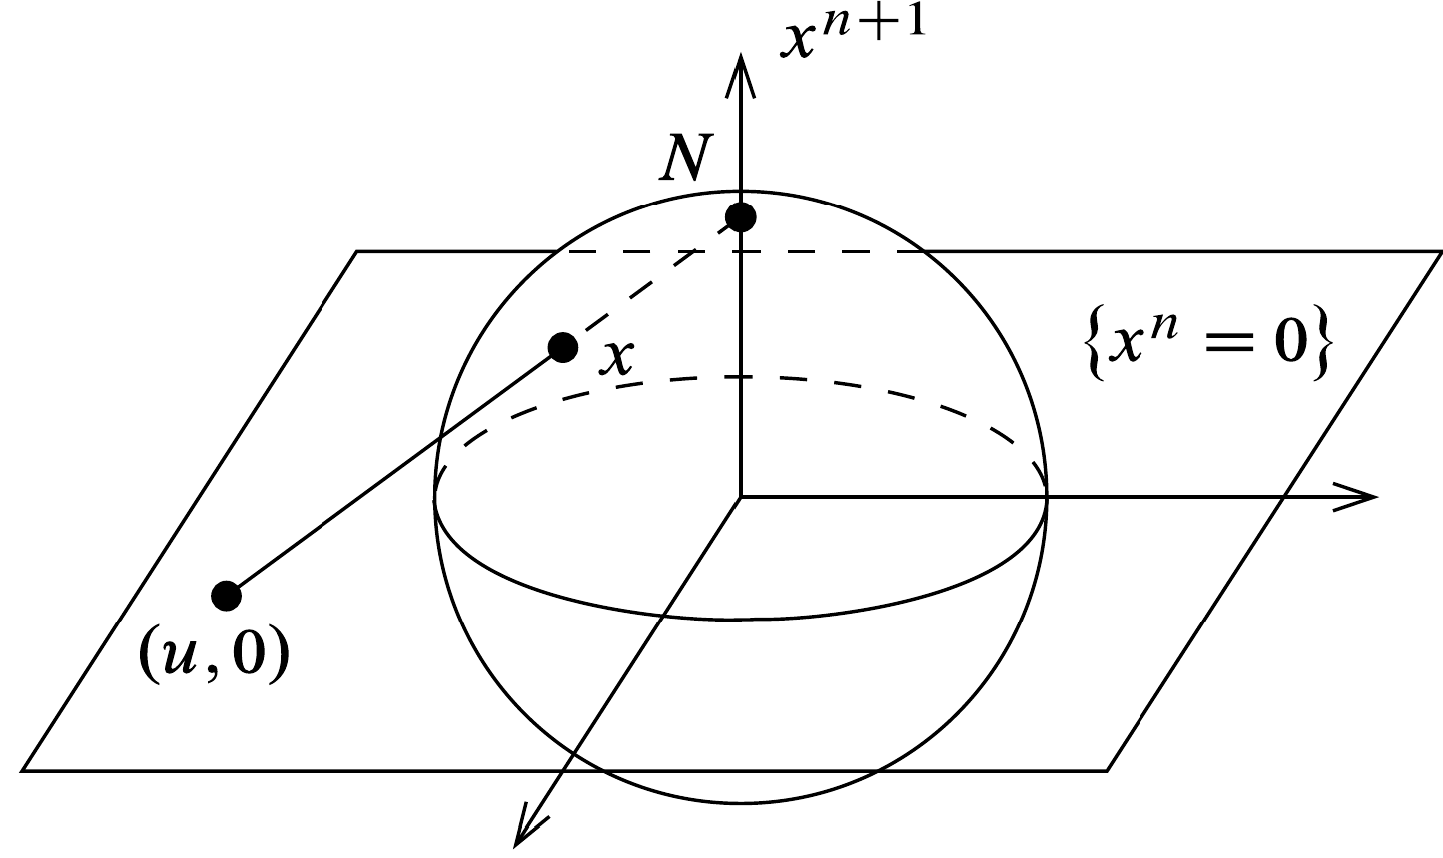
\includegraphics[scale=0.36]{1.png}
\end{center}
    \begin{proof}

        (1) Define the line passing through $N$ and $x$ by
        \[
            L(t) = N + t(x - N) = u(t)
        \]
        Consider the intersection between $L(t)$ and the linear subspace of $\bb{R}^{n + 1}$ where $x^{n + 1} = 0$, we have 
        \[
            u(t) = (tx^1, \dots ,tx^n, 1 + t(x^{n + 1} - 1)) = (u^1,\dots, u^n, 0)
        \]
        The $(n+1)-$term implies that $t = \dfrac{1}{1 - x^{n + 1}}$, thus we have 
        \[
            u(t) = \frac{(x^1,\dots,x^n)}{1 - x^{n + 1}} = \sigma(x)
        \]
        (2) Let $u = (u^1,\dots, u^n) \in \bb{R}^{n}$, it suffices to prove that there exists $(x^1,\dots,x^{n+1}) \in \bb{S}^n \backslash\{N\}$ satisfying 
        \[
            u^i = \frac{x^i}{1 - x^{n + 1}} \text{ for all }i = 1,\dots, n.
        \]
        Let $|u|^2 = \sum (u^i)^2$, it follows that 
        \begin{align*}
            |u|^2 & = \frac{\sum (x^i)^2}{(1 - x^{n + 1})^2}= \frac{1 - (x^{n + 1})^2}{(1 - x^{n + 1})^2} = \frac{1 + x^{n + 1}}{1 - x^{n + 1}} = \frac{2}{1 - x^{n + 1}} - 1\\
            &\lra x^{n + 1} = \frac{|u|^2 - 1}{|u|^2 + 1} 
        \end{align*}
        Since $-1 < \dfrac{|u|^2 - 1}{|u|^2 + 1} < 1$, set $x^{n + 1}= \dfrac{|u|^2 - 1}{|u|^2 + 1} $ and $x^i = \dfrac{2u^i}{|u|^2 + 1}$. Thus $\sigma$ is surjective onto $\bb{R}^n$.
        
        To prove that  $\sigma$ is injective, suppose $\sigma(x) = \sigma(y)$,  we have
        \begin{align*}
            \frac{x^i}{1 - x^{n + 1}} = \frac{y^i}{1 - y^{n+ 1}} &\ra \frac{\sum (x^i)^2}{( 1 - x^{n + 1})^2}=\frac{\sum (y^i)^2}{( 1 - y^{n + 1})^2}\\
            &\lra \frac{1 + x^{n + 1}}{1 - x^{n + 1}} = \frac{1 + y^{n + 1}}{1 - y^{n +1}}\\
            &\lra \frac{2}{1 - x^{n + 1}} - 1 =\frac{2}{1 - y^{n + 1}} - 1\\
            &\lra\frac{2}{1 - x^{n + 1}} = \frac{2}{1 - y^{n + 1}}\\
            &\lra 1 - x^{n + 1} = 1 - y^{n + 1},
        \end{align*}
        which implies $x^{n + 1} = y^{n + 1}$ and hence $x^i = y^i$ for all $i = 1,\dots,n$. Therefore $\sigma$ is bijective and its inverse satisfies 
        $$
        \sigma^{-1}\left(u^1, \ldots, u^n\right)=\frac{\left(2 u^1, \ldots, 2 u^n,|u|^2-1\right)}{|u|^2+1}
        $$
        We will verify that $\sigma^{-1}(u) \in \bb{S}^{n}$ for all $u$. Let $(x^i) = \sigma^{-1}(u)$, since we have 
        \[
            \sum (x^i)^2 = \frac{\sum(2u^i)^2 + (|u|^2 - 1)^2}{(|u|^2 + 1)^2} = \frac{4|u|^2 + ( |u|^2 - 1)^2}{(|u|^2 + 1)^2} = \frac{(|u|^2 + 1)^2}{(|u|^2 + 1)^2} = 1
        \]
        Thus $\sigma^{-1}$ maps every point in $\bb{R}^{n}$ into the sphere $\bb{S}^n$.
        (3) By the definition of $\tilde{\sigma}$, it can be written as 
        \[
            \tilde{\sigma}(x^1,\dots,x^{n + 1}) = \frac{(x^1,\dots,x^{n})}{1 + x^{n + 1}},
        \]
        and the same computation shows that $\tilde{\sigma}$ is bijective. Let $u = (u^i) \in \bb{R}^n\backslash\{0\}$ , the composition $\tilde{\sigma}\circ \sigma^{-1}: \bb{R}^n\backslash\{0\} \to \bb{R}^n\backslash\{0\}$ is computed by expressing 
        \begin{align*}
            \tilde{\sigma}\circ \sigma^{-1}(u) &=\tilde{\sigma}\left(\frac{2 u^1}{|u|^2+1}, \ldots, \frac{2 u^n}{|u|^2+1},\frac{|u|^2-1}{|u|^2+1}\right)\\
            &= \frac{(u^1,\dots, u^n)}{|u|^2}.
        \end{align*}
        Since $\tilde{\sigma}\circ \sigma^{-1}$ is smooth and a diffeomorphism, $\sigma$ and $\tilde{\sigma}$ are compatible. Moreover, since the union of their domains covers entire $\bb{S}^n$, then they form an atlas which generates a smooth structure on $\bb{S}^n$.
        
    \end{proof}
\begin{problem}
    By identifying $\mathbb{R}^2$ with $\mathbb{C}$, we can think of the unit circle $\mathbb{S}^1$ as a subset of the complex plane. An angle function on a subset $U \subseteq \mathbb{S}^1$ is a continuous function $\theta: U \rightarrow \mathbb{R}$ such that $e^{i \theta(z)}=z$ for all $z \in U$. Show that there exists an angle function $\theta$ on an open subset $U \subseteq \mathbb{S}^1$ if and only if $U \neq \mathbb{S}^1$. For any such angle function, show that ($U, \theta$) is a smooth coordinate chart for $\mathbb{S}^1$ with its standard smooth structure.
\end{problem}
\begin{proof}
    ($\ra$) Suppose there exists an angle function $\theta:\bb{S}^1 \to \bb{R}$ which is continuous. We aim to show that $\theta$ is discontinuous at $z = 1$. If we write $z = e^{i\pi \phi}$ then it follows that $\theta = \pi\phi + k2\pi$, where $k$ is some integer. Since $\theta$ is continuous, $k$ must be fixed. Let 
    \[
        a_n = e^{i\pi/n} \text{ and }b_n = e^{i(2\pi - 1/n)}
    \]
    Then we have 
    \[
        \nlim \theta(a_n) = \theta(0) = k2\pi\text{ and }\nlim\theta(b_n) =  \theta(2\pi) = 2\pi + k2\pi
    \]
    Since $2\pi \neq 0$, $\theta$ is not continuous at $z = 1$, hence there is no angle function for the case $U = \bb{S}^1$. We define $\alpha(z)$  as a unique function satisfying $z = e^{i\pi\alpha(z)}$ and $\alpha(z) \in [0,2\pi)$.
    
    If $U \neq \bb{S}^1$. In case that $1 \in U$, since there must exsits $z_0 \neq 1$ and $z_0 \notin U$. Since $\alpha$ is continuous, we choose  $\theta$ satisfying
    \begin{align*}
         \theta(z) = \alpha(z) , ( \alpha(z)  < \alpha(z_0) ) \text{ and }\\
         \theta(z)=2\pi -  \alpha(z) , ( \alpha(z)  \geq \alpha(z_0) )
    \end{align*}
    If  $1 \notin U$, we choose $\theta(z) = \alpha(z)$ for all $z\in U$.  

    Since $\theta$ is continuous and a homeomorphism on from open subset $U \subset \bb{S}^1$ onto an open interval $\theta(U)$, the pair $(U,\theta)$ is a smooth coordinate chart for $\bb{S}^1$ with its standard smooth structure.
\end{proof}
\begin{problem}
     Complex projective $n$-space, denoted by $\mathbb{C P}^n$, is the set of all 1-dimensional complex-linear subspaces of $\mathbb{C}^{n+1}$, with the quotient topology inherited from the natural projection $\pi: \mathbb{C}^{n+1} \backslash\{0\} \rightarrow \mathbb{C} \mathbb{P}^n$. Show that $\mathbb{C} \mathbb{P}^n$ is a compact $2 n$-dimensional topological manifold, and show how to give it a smooth structure analogous to the one we constructed for $\mathbb{R P}^n$. (We use the correspondence
$$
\left(x^1+i y^1, \ldots, x^{n+1}+i y^{n+1}\right) \leftrightarrow\left(x^1, y^1, \ldots, x^{n+1}, y^{n+1}\right)
$$
to identify $\mathbb{C}^{n+1}$ with $\mathbb{R}^{2 n+2}$.) (Used on pp. 48, 96, 172, 560, 561.)
\end{problem}
\begin{proof}
    Suppose $\bb{S}^n$ is an $n$-dimensional sphere, it suffices to prove the restriction map $$\pi|_{\bb{S}^n}: \bb{S}^n \to \bb{CP}^n$$ is continuous and surjective. For the sake of condition, we assume to write $\pi$ instead of $\pi|_{\bb{S}^n}$. Given $z \in \bb{CP}^n$, by the definiton of projective space, $z$ is an equivalent class satisfying
    \[
        [z^0: \dots : z^n] \sim [\lambda z^0: \dots :\lambda z^n]
    \]
    for all nonzero complex number $\lambda$. To prove $\pi$ is surjective, let $[z] \in \bb{CP}^n$ be abitrary, one can rewrite 
    \[
        [z] = [z^0: \dots : z^n] \sim \left[\frac{z^0}{|z|}: \dots : \frac{z^n}{|z|}\right]
    \]
    Since we have 
    \[
        \sum \dfrac{(z^i)^2}{|z|^2} = \frac{|z|^2}{|z|^2} = 1
    \]
    then $\left(\dfrac{z^0}{|z|}: \dots : \dfrac{z^n}{|z|}\right) \in \bb{S}^n$ and hence it follows that $\pi\left(\dfrac{z^0}{|z|}: \dots : \dfrac{z^n}{|z|}\right) = [z]$. Since the natural projection  $\pi: \mathbb{C}^{n+1} \backslash\{0\} \rightarrow \mathbb{C} \mathbb{P}^n$ is already continuous, the its restriction on closed subset $\bb{S}^n$ is also continuous. Since $\bb{S}^{n}$ is closed and bounded in $\bb{C}^{n + 1}$ by the corresponding identify $\bb{C}^{n + 1}$ with $\bb{R}^{2n + 2}$, by the Heine-Borrel theorem, $\bb{S}^n$ is compact. And since $\pi_{\bb{S}^n}(\bb{CP}^n) =\bb{S}^n$, $\bb{CP}^n$ is a compact.

    To prove $\bb{CP}^n$ is locally Euclidean, for each $i = 0,\dots,n$, let $\tilde{U_i}\subset \bb{C}^{n + 1}$ be the subset containing all points $x \in \bb{C}^{n + 1}$ satisfying $x^{i} \neq 0$ and $\varphi_i: U_i \to \bb{C}^{n}$ be the local chart (where $U_i = \pi(\tilde{U_i})$) satisfying
    \[  
        \varphi[z^0: \dots : z^n] = \left(\frac{z^0}{z^i},\dots,\frac{z^{i -1}}{z^{i}},\frac{z^{i + 1}}{z^{i}}, \dots,\frac{z^n}{z^i}\right).
    \]
    This map is well-defined since the left-hand side remains if we replace $[z^1: \dots : z^n]$ by $\lambda[z^1: \dots : z^n]$. To prove $\varphi_i$ is injective, suppose $\varphi_i[a] = \varphi_i[b]$, then we have 
    \[  
        \frac{a^j}{a^i} = \frac{b^j}{b^i} \text{ for all }j = 0, \dots,n + 1
    \]
    Let $\lambda = \dfrac{a^i}{b^i}$ be fixed, it follows that $a^j = \lambda b^j$ for all $j = 0,\dots, n + 1$, hence $[a] = [b]$. To prove $\varphi_i$ is surjective, if $x \in \bb{C}^n$, we choose $[z] \in \bb{CP}^n$ satisfying $z^j = x^{j - 1}$ for all $j \neq i$ and $z^i = 1$, this implies $\varphi_{i}[z] =  x$. Therefore $\varphi_i$ is bijective. Moreover, $\varphi$ is smooth and its inverse given by
    \[
        \varphi_i^{-1}(x^i) = [x^0,\dots,x^{i - 1}, 1, x^{i + 1},\dots,x^n]
    \]
    is also smooth. Thus $\varphi_i$ is homeomorphism and $\bb{C}^n \cong \bb{R}^{2n}$ implies that $\bb{CP}^n$ is locally $2n$-dimensional Euclidean. In particular, since $\varphi_i$  is diffeomorphism, it follows that $(U_i,\varphi_i)$ is smooth local chart and they are parwise compatible since a composition of two diffeomorphism is again a diffeomorphism. Hence, the atlas $\{(U_i,\varphi_i)\}$ defines a smooth structure on $\bb{CP}^n$.

    To prove $\bb{CP}^n$ is Hausdorff, let $[a],[b]$ be distinct equivalence classes in $\bb{CP}^n$, which means $[a] \neq [b]$, pushed forward by $\varphi_i$, where $i$ is the non-negative integer satisfying $a^i, b^i \neq 0$. By consider two open disks 
    \begin{align*}
        &\mc{D}_{\varphi_i(a)} = \{z \in \bb{C}^n \mid |z - \varphi_i(a)| < \ep\} \text{ and }\\
        &\mc{D}_{\varphi_i(b)} = \{z \in \bb{C}^n \mid |z - \varphi_i(b)| < \ep\}
    \end{align*}
    where $\ep > 0$ satisfies $\ep < \dfrac{|\varphi(a) - \varphi(b)|}{2}$ implying $\mc{D}_{\varphi(a)} \cap \mc{D}_{\varphi(b)} = \varnothing$. Since $\varphi_i$ is homeomorphism, then any distinct points in $\bb{CP}^n$ can be seperated by two open disjoint neighborhoods, which is $\mc{D}_{\varphi(a)}$ and $\mc{D}_{\varphi(b)}$ in this case. Therefore $\bb{CP}^n$ is Hausdorff.

    The fact that $ \bb{C}^n$ is second-countable and $\{(U_i,\varphi_i)\}$ is a smooth structure implies that $\bb{CP}^n$ is also second-countable. In conclusion, $\bb{CP}^n$ is a compact $2 n$-dimensional topological manifold, as desired.
    

\end{proof}
\begin{problem}
     Let $k$ and $n$ be integers satisfying $0<k<n$, and let $P, Q \subseteq \mathbb{R}^n$ be the linear subspaces spanned by $\left(e_1, \ldots, e_k\right)$ and $\left(e_{k+1}, \ldots, e_n\right)$, respectively, where $e_i$ is the $i$ th standard basis vector for $\mathbb{R}^n$. For any $k$-dimensional subspace $S \subseteq \mathbb{R}^n$ that has trivial intersection with $Q$, show that the coordinate representation $\varphi(S)$ constructed in Example 1.36 is the unique $(n-k) \times k$ matrix $B$ such that $S$ is spanned by the columns of the matrix $\binom{I_k}{B}$, where $I_k$ denotes the $k \times k$ identity matrix.
\end{problem}
\begin{problem}
    Let $M=\overline{\mathbb{B}}^n$, the closed unit ball in $\mathbb{R}^n$. Show that $M$ is a topological manifold with boundary in which each point in $\mathbb{S}^{n-1}$ is a boundary point and each point in $\mathbb{B}^n$ is an interior point. Show how to give it a smooth structure such that every smooth interior chart is a smooth chart for the standard smooth structure on $\mathbb{B}^n$. [Hint: consider the map $\pi \circ \sigma^{-1}: \mathbb{R}^n \rightarrow \mathbb{R}^n$, where $\sigma: \mathbb{S}^n \rightarrow \mathbb{R}^n$ is the stereographic projection (Problem 1-7) and $\pi$ is a projection from $\mathbb{R}^{n+1}$ to $\mathbb{R}^n$ that omits some coordinate other than the last.]    
\end{problem}
\begin{problem}
    Prove Proposition 1.45 (a product of smooth manifolds together with one smooth manifold with boundary is a smooth manifold with boundary).
\end{problem}